\section{Protocol Specifications}


\begingroup
\setlength{\tabcolsep}{10pt} % Default value: 6pt
\renewcommand{\arraystretch}{1.5} % Default value: 1
\begin{table}[h]
    \centering
    \caption{G-Code definitions}
    \label{tab:g-definitions}
    \begin{tabular}{p{0.1\textwidth}p{0.8\textwidth}}
    \toprule
    G-Code & Definition \\ \midrule
    \texttt{G1} & Move one or more actuators to specified positions at a given optional speed. \\
    \texttt{G4} & Pause or dwell. Halts the machine for the specified duration. \\
    \texttt{G28} & Move actuators to origin position. \\
    \texttt{G28.1} & Move actuators to target position. \\
    \texttt{G90} & Set absolute positioning mode. All subsequent movements are interpreted as absolute positions. This is the default mode. \\
    \texttt{G91} & Set relative positioning mode. All subsequent movements are interpreted as displacements from the current position. \\
    \texttt{G92} & Set origin position. \\
    \texttt{G92.1} & Set target position. This may be a position of interest. \\ \bottomrule
    \end{tabular}
\end{table}
\endgroup

\begingroup
\setlength{\tabcolsep}{10pt} % Default value: 6pt
\renewcommand{\arraystretch}{1.5} % Default value: 1
\begin{table}[h]
    \centering
    \caption{M-Code definitions}
    \label{tab:m-definitions}
    \begin{tabular}{ll}
    \toprule
    M-Code & Definition \\ \midrule
    \texttt{M00} & Stop program \\
    \texttt{M85} & Maximum command wait time. \\
    \texttt{M114} & Report current position of the actuators. \\
    \texttt{M301} & Set PID parameters. \\
    \texttt{M303} & Initiate autotuning process for the PID parameters. \\
    \texttt{M355} & Report current status of robot parameters. \\
    \texttt{M500} & Save parameters to EEPROM. \\
    \texttt{M501} & Load parameters from EEPROM. \\
    \texttt{M502} & Reset parameters saved in EEPROM to defaults. \\
    \texttt{M503} & Display the saved configuration in EEPROM. \\ \bottomrule
    \end{tabular}
\end{table}
\endgroup

\newcommand{\prompt}{\texttt{> }}

\begingroup
\setlength{\tabcolsep}{10pt}
\renewcommand{\arraystretch}{1.5}
\begin{table}[h]
    \centering
    \caption{G-Codes usage}
    \label{tab:g-codes-usage}
    \begin{tabular}{p{0.1\textwidth}p{0.47\textwidth}p{0.28\textwidth}}
    \toprule
    Code & Usage & Example \\ \midrule
    \texttt{G1}  & \gcodeinline/G1 <id><pos> [F<speed,255>]/ & \prompt\gcodeinline/G1 A100.0/\\
    \texttt{G4}  & \gcodeinline/G4 P<millis>|S<secs>/ & \prompt\gcodeinline/G4 P3000/\\
    \texttt{G20} & \gcodeinline/G20/ & \prompt\gcodeinline/G20/\\
    \texttt{G21} & \gcodeinline/G21/ & \prompt\gcodeinline/G21/ \\
    \texttt{G28} & \gcodeinline/G28 [<id,A B C I J K>]/ & \prompt\gcodeinline/G28 A B C/\\
    \texttt{G28} & \gcodeinline/G28.1 [<id,A B C I J K>]/ & \prompt\gcodeinline/G28.1 J K/\\
    \texttt{G90} & \gcodeinline/G90/ & \prompt\gcodeinline/G90/\\
    \texttt{G91} & \gcodeinline/G91/ & \prompt\gcodeinline/G91/\\
    \texttt{G92} & \gcodeinline/G92 [<id,A B C I J K><pos,0>]/& \prompt\gcodeinline/G92 A-100.0 I5.0/\\
    \texttt{G92.1} & \gcodeinline/G92.1 [<id, A B C I J K><pos,0>]/& \prompt\gcodeinline/G92.1 B250.0/\\
    \bottomrule
    \end{tabular}
\end{table}
\endgroup

\begingroup
\setlength{\tabcolsep}{10pt}
\renewcommand{\arraystretch}{1.5}
\begin{table}[h]
    \centering
    \caption{M-Codes usage}
    \caption*{Note that only commands with parameters are explained. All others can be used by simply entering the code.}
    \label{tab:m-codes-usage}
    \begin{tabular}{p{0.1\textwidth}p{0.5\textwidth}p{0.25\textwidth}}
    \toprule
    Code & Usage & Example \\ \midrule
    \texttt{M85} & \gcodeinline/M85 P<millis,5000>|S<secs,5>/ & \prompt\gcodeinline/M85 S3/ \\
    \texttt{M301} & \gcodeinline/M301 [P<kp,0>] [I<ki,0>] [D<kd,0>]/ & \prompt\gcodeinline/M301 P1000 I0.5/ \\
    \texttt{M500} & \gcodeinline/M500 <optn>/ & \prompt\gcodeinline/M500 T P/ \\
    \texttt{M502} & \gcodeinline/M502 <optn>/ & \prompt\gcodeinline/M502 I J K/\\
    \bottomrule
    \end{tabular}
\end{table}
\endgroup

\begingroup
\setlength{\tabcolsep}{10pt}
\renewcommand{\arraystretch}{1.5}
\begin{table}[h]
    \centering
    \caption{Code parameters}
    \label{tab:code-parameters}
    \begin{tabular}{p{0.2\textwidth}p{0.7\textwidth}}
    \toprule
    Parameter & Meaning \\ \midrule
    \texttt{<id>} & Actuator identification letter: \texttt{A}, \texttt{B}, \texttt{C}, \texttt{I}, \texttt{J} or \texttt{K}. \\
    \texttt{<pos>} & Position number. \\
    \texttt{<kp>} & Proportional constant. \\
    \texttt{<ki>} & Integral constant. \\
    \texttt{<kd>} & Derivative constant. \\
    \texttt{<speed>} & Maximum speed of actuator as integer number from \texttt{50} to \texttt{255}. \\
    \texttt{<millis>} & Milliseconds as integer number. \\
    \texttt{<secs>} & Seconds as integer number. \\
    \texttt{<optn>} & Parameter of the robot. \texttt{T} for PID tuning constants; \texttt{A}, \texttt{B}, \texttt{C}, \texttt{I}, \texttt{J} or \texttt{K} for position of given actuator; \texttt{P} for \textbf{all} actuator positions\\
    \texttt{<...,VALUE>} & Default value. \\
    \texttt{[...]} & Optional parameter. If omitted, default value will be used. \\
    \bottomrule
    \end{tabular}
\end{table}
\endgroup

\section{Command Line Application}

\subsection{Architecture}

\begin{figure}[]
    \centering
    \includesvg[width=0.95\textwidth]{firmware-uml}
    \caption{Relationships of control system components}
    \label{fig:firmware-uml}
\end{figure}

\begin{figure}[]
    \centering
    \includesvg[width=0.95\textwidth]{system-flowchart}
    \caption{System flowchart}
    \label{fig:system-flowchart}
\end{figure}


\subsection{Usage}

\begin{figure}[]
    \centering
    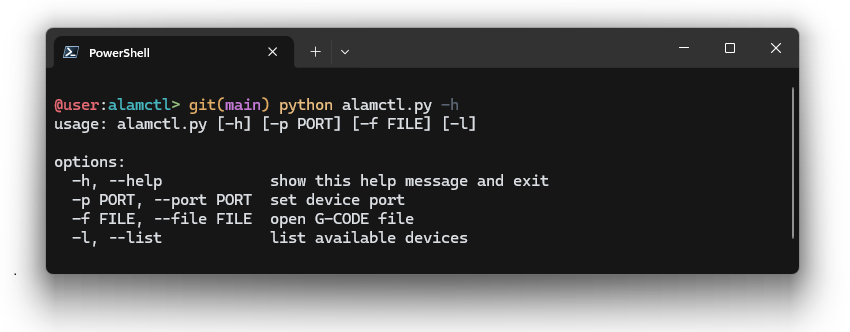
\includegraphics[width=0.95\textwidth]{cli-usage}
    \caption{Command line usage}
    \label{fig:cli-usage}
\end{figure}

\begin{figure}[]
    \centering
    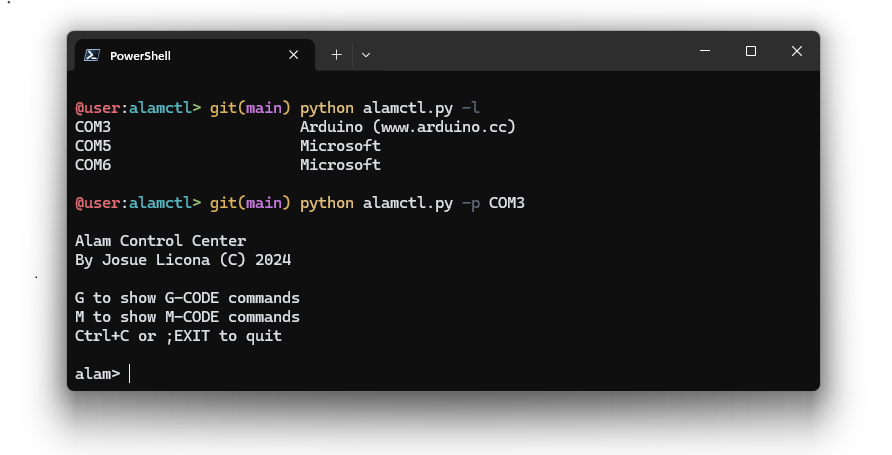
\includegraphics[width=0.95\textwidth]{cli-connection}
    \caption{Command line connection}
    \label{fig:cli-connection}
\end{figure}

\begin{figure}[]
    \centering
    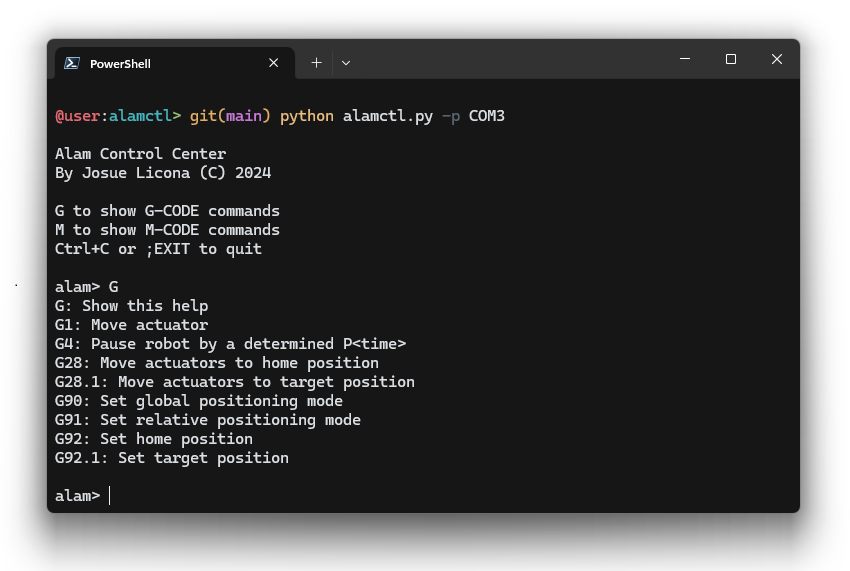
\includegraphics[width=0.95\textwidth]{cli-manual}
    \caption{Command line manual input}
    \label{fig:cli-manual}
\end{figure}

\begin{figure}[]
    \centering
    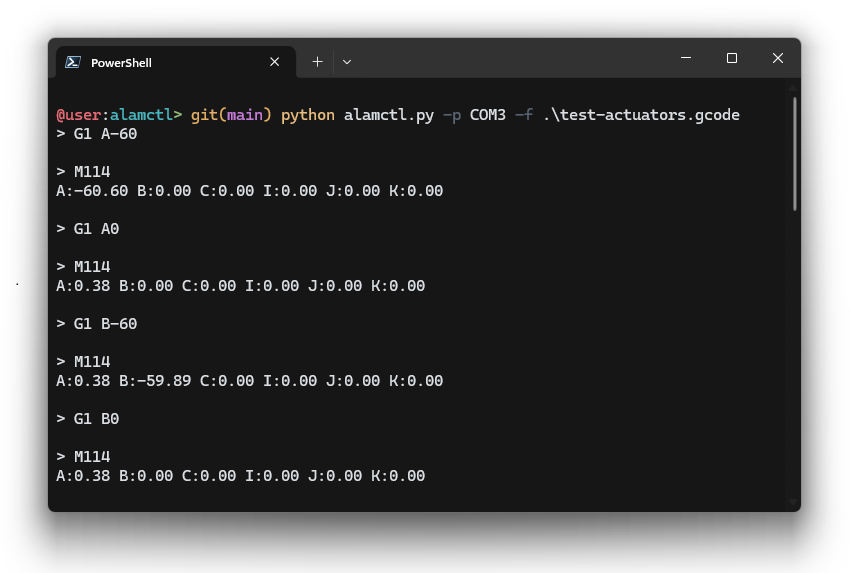
\includegraphics[width=0.95\textwidth]{cli-file}
    \caption{Command line file parsing}
    \label{fig:cli-file}
\end{figure}

\section{PID Control and Tuning}

\subsection{Test Data}
\begin{figure}[h]
    \centering
    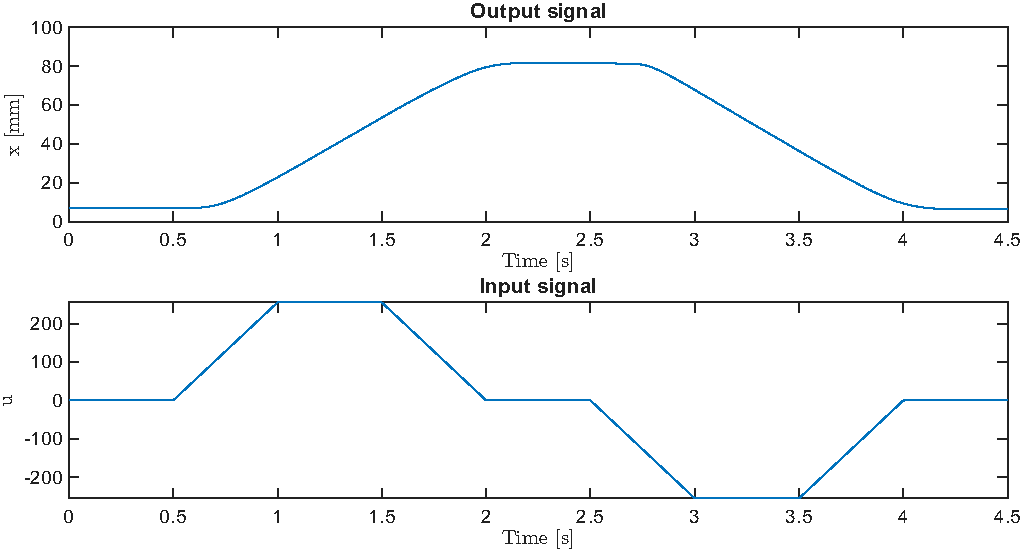
\includegraphics[page=1,width=0.95\textwidth]{input-output-signals}
    \caption{Input and output signals}
    \label{fig:io-signals}
\end{figure}

\subsection{System Identification}

\begin{figure}[h]
    \centering
    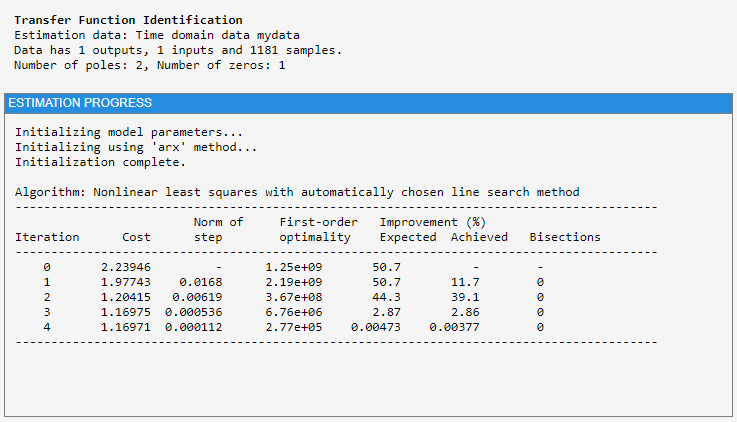
\includegraphics[width=0.7\textwidth]{tf-ident-process}
    \caption{Transfer function identification in MATLAB}
    \label{fig:tf-indent-process}
\end{figure}

\begin{figure}[h]
    \centering
    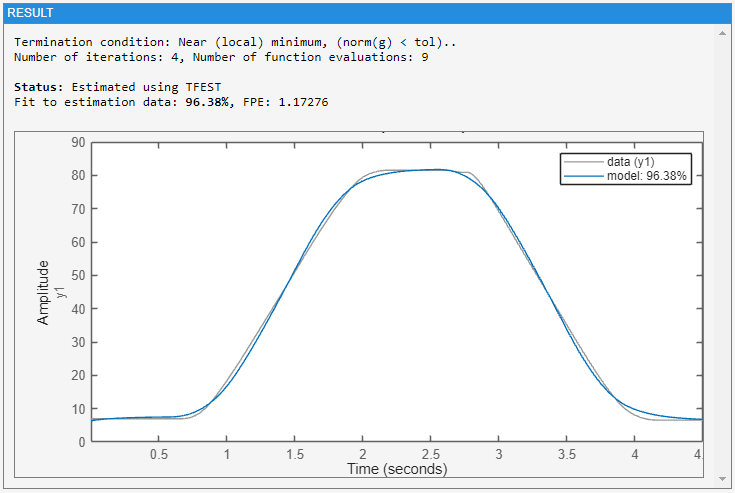
\includegraphics[width=0.7\textwidth]{tf-ident-result}
    \caption{Transfer function model in MATLAB}
    \label{fig:tf-result}
\end{figure}


\begin{equation}
    \label{eq:tf}
    tf=\frac{(4.808-4.596z^{-1})\times10^{-4}}{1-1.982z^{-1}+0.9824z^{-2}}
\end{equation}


\subsection{PID Tuning}

\begin{equation}
    C = Kp + Ki * \frac{Ts}{z-1}
\end{equation}

\begin{table}[h]
    \centering
    \caption{PID Tunings}
    \label{tab:pid-tunings}
    \begin{tabular}{ll}
    \toprule
    Property & Value \\
    \midrule
    Proportional constant, $Kp$  & 21.4 \\
    Integrative constant, $Ki$ & 1.97 \\
    Sample time, $Ts$ & $0.00381$s \\
    \bottomrule
    \end{tabular}
\end{table}

\begin{figure}[h]
    \centering
    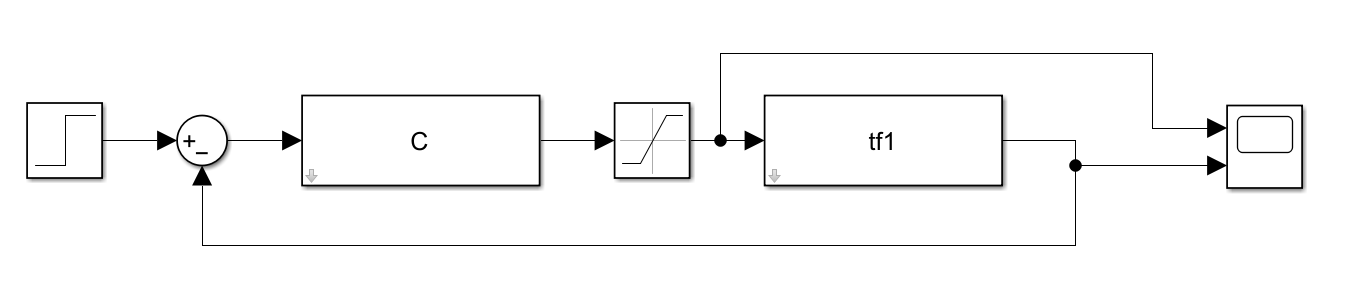
\includegraphics[width=\textwidth]{system-blocks}
    \caption{Blocks diagram of control system}
    \label{fig:system-blocks}
\end{figure}

\begin{figure}[h]
    \centering
    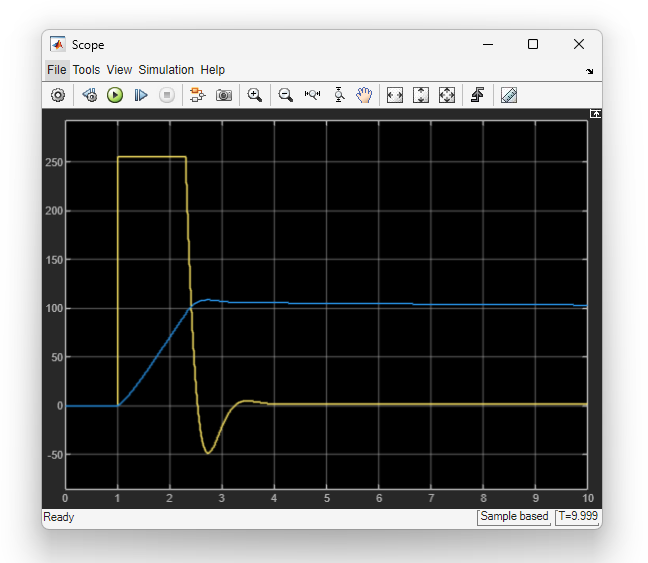
\includegraphics[width=0.6\textwidth]{system-response}
    \caption{System response of simulation in Simulink}
    \label{fig:system-response}
\end{figure}